\documentclass[tikz,14pt,border=10pt]{standalone}
\usepackage[T1]{fontenc}
\usepackage[latin1]{inputenc}
\usepackage[english]{babel}
\usepackage{textcomp}
\usetikzlibrary{shapes,patterns,arrows,calc,decorations.pathreplacing,positioning,graphs}
\usepackage{pgfmath}
\usepackage{tikz}
\usetikzlibrary{calc}
\usepackage{amsmath}


\begin{document}

\begin{tikzpicture}
\node (pic) at (0,0) {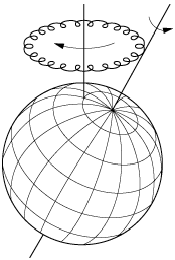
\includegraphics[height=5cm]{./../pic/praezession}};

\node (a1) at ($(pic)+ (-3mm,14mm)$) {$\omega_p$};
\def\offset{20mm}
\node[coordinate] (a2) at  ($(pic)+ (\offset,20mm)$) {};
\node[coordinate] (a3) at  ($(pic)+ (\offset,-20mm)$) {};
\draw[-latex,color=red] (a3) -- (a2) node[left,near end] {$\vec{B}$};
\end{tikzpicture}

\end{document}